\documentclass[10pt]{article}
\usepackage[a4paper,margin=19mm]{geometry}
\usepackage{amsmath,amssymb,booktabs,xcolor,tikz,hyperref}
\definecolor{blueink}{HTML}{145B79}
\hypersetup{colorlinks=true,urlcolor=blueink}
\setlength{\parindent}{0pt}\setlength{\parskip}{4pt}
\newcommand{\head}[1]{\smallskip{\large\bfseries\color{blueink}#1}\par}
\begin{document}
{\small\sffamily\color{blueink} DISCRETE GEOMETRY\quad /\quad RESEARCH NOTE\hfill 27 NOVEMBER 2026}\par
{\LARGE\bfseries Two more eight-point planar crescents}\par
\textit{Leo Gao $\cdot$ AI-assisted research note}
\medskip

Eight points form a crescent if no three lie on a line, no four lie on a circle, and their 28 pairwise distances occur with multiplicities $1,2,\ldots,7$. The three examples in Jafari and Amin's 2016 Table 11 do not exhaust the possibilities. The following two are not similar to any of those three, or to each other.

\head{The construction}
Choose $r=\sqrt6$ or $r=-\sqrt6$. Read $(x,y)$ in the display as the \emph{Euclidean} point $(x,\sqrt3\,y)$. In order from $P_0$ to $P_7$, take
\[
\begin{array}{rcl@{\qquad}rcl}
P_0&=&(0,0), &P_4&=&(3-r,-r-1),\\
P_1&=&(-2r,4),&P_5&=&(3,3),\\
P_2&=&(3-r,r+5),&P_6&=&(r+6,r+4),\\
P_3&=&(6,0),&P_7&=&(-2r-3,1).
\end{array}
\]
\centerline{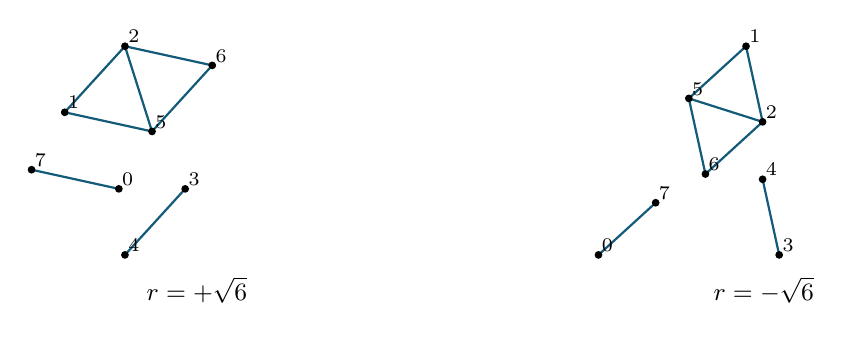
\begin{tikzpicture}[x=1cm,y=1cm]
\draw[blueink,thick] (1.30884,1.28872)--(0.20000,1.53186);
\draw[blueink,thick] (0.62113,2.26128)--(1.38612,3.10000);
\draw[blueink,thick] (0.62113,2.26128)--(1.72998,2.01814);
\draw[blueink,thick] (1.38612,3.10000)--(1.72998,2.01814);
\draw[blueink,thick] (1.38612,3.10000)--(2.49497,2.85686);
\draw[blueink,thick] (2.15111,1.28872)--(1.38612,0.45000);
\draw[blueink,thick] (1.72998,2.01814)--(2.49497,2.85686);
\fill (1.30884,1.28872) circle (1.4pt) node[above right,inner sep=1pt,font=\scriptsize] {0};
\fill (0.62113,2.26128) circle (1.4pt) node[above right,inner sep=1pt,font=\scriptsize] {1};
\fill (1.38612,3.10000) circle (1.4pt) node[above right,inner sep=1pt,font=\scriptsize] {2};
\fill (2.15111,1.28872) circle (1.4pt) node[above right,inner sep=1pt,font=\scriptsize] {3};
\fill (1.38612,0.45000) circle (1.4pt) node[above right,inner sep=1pt,font=\scriptsize] {4};
\fill (1.72998,2.01814) circle (1.4pt) node[above right,inner sep=1pt,font=\scriptsize] {5};
\fill (2.49497,2.85686) circle (1.4pt) node[above right,inner sep=1pt,font=\scriptsize] {6};
\fill (0.20000,1.53186) circle (1.4pt) node[above right,inner sep=1pt,font=\scriptsize] {7};
\node[font=\small] at (2.3000,0) {$r=+\sqrt6$};
\draw[blueink,thick] (7.40000,0.45000)--(8.12635,1.11250);
\draw[blueink,thick] (9.27383,3.10000)--(9.48440,2.13971);
\draw[blueink,thick] (9.27383,3.10000)--(8.54748,2.43750);
\draw[blueink,thick] (9.48440,2.13971)--(8.54748,2.43750);
\draw[blueink,thick] (9.48440,2.13971)--(8.75805,1.47721);
\draw[blueink,thick] (9.69497,0.45000)--(9.48440,1.41029);
\draw[blueink,thick] (8.54748,2.43750)--(8.75805,1.47721);
\fill (7.40000,0.45000) circle (1.4pt) node[above right,inner sep=1pt,font=\scriptsize] {0};
\fill (9.27383,3.10000) circle (1.4pt) node[above right,inner sep=1pt,font=\scriptsize] {1};
\fill (9.48440,2.13971) circle (1.4pt) node[above right,inner sep=1pt,font=\scriptsize] {2};
\fill (9.69497,0.45000) circle (1.4pt) node[above right,inner sep=1pt,font=\scriptsize] {3};
\fill (9.48440,1.41029) circle (1.4pt) node[above right,inner sep=1pt,font=\scriptsize] {4};
\fill (8.54748,2.43750) circle (1.4pt) node[above right,inner sep=1pt,font=\scriptsize] {5};
\fill (8.75805,1.47721) circle (1.4pt) node[above right,inner sep=1pt,font=\scriptsize] {6};
\fill (8.12635,1.11250) circle (1.4pt) node[above right,inner sep=1pt,font=\scriptsize] {7};
\node[font=\small] at (9.5000,0) {$r=-\sqrt6$};
\end{tikzpicture}
}
\centerline{\small Seven blue segments have the most frequent length.}

\head{Exact distance check}
The squared lengths in multiplicity order are
\[
72,\quad108+24r,\quad180+72r,\quad72+24r,\quad36,\quad108+36r,\quad36+12r.
\]
Indeed, subtract the displayed pairs and use $q(x,y)=x^2+3y^2$ and $r^2=6$. In lexicographic pair order $01,02,\ldots,67$, the resulting multiplicity labels are
\[
\mathtt{1255567726765637767546434743}.
\]
They are genuinely distinct, as the certificate below also verifies.

\head{A one-prime certificate of general position}
Reduce the integer ring $\mathbb Z[r]/(r^2-6)$ modulo $19$ by sending $r$ to $5$. In the displayed point order, the product of the 56 triple determinants with rows $(1,x,y)$ reduces to $14$. The product of the 70 quadruple determinants with rows $(1,x,y,q(x,y))$ reduces to $3$. The product of the 21 differences of squared lengths (smaller multiplicity index first) reduces to $16$. These nonzero residues prove that no factor vanishes in the number field, hence under either real embedding. Noncollinearity and nonconcyclicity follow because $(x,y)$ are invertible affine coordinates and $q$ is the Euclidean squared norm. The small standard-library checker reproduces the three residues and every distance equality.

\newpage
{\large\bfseries Why these are different shapes}\par
The ratio $s_2/s_1$ of the squared lengths with multiplicities two and one equals $3/2+r/3$. Its values distinguish the two conjugates. Their squared-distance ratio field is $\mathbb Q(\sqrt6)$. By contrast, Pal\'asti's triangular-lattice example has rational ratios. Both other configurations in \href{https://doi.org/10.4236/ojdm.2016.63012}{Jafari--Amin, Table 11} have ratios in $\mathbb Q(\sqrt{57})$: their first Cartesian coordinates lie in that field and their second coordinates in $\sqrt3\,\mathbb Q(\sqrt{57})$. These quadratic fields are different. Thus there are at least five similarity classes of eight-point planar crescents. This distinguishes the pair from those three published entries; it does not classify every order-eight configuration.

\head{Exactly two shapes realize this edge pattern}
Here is a short converse, independent of the search. Normalize $s_1=1$, and write $v=s_7$. The word forces the opposite vertex pairs $(0,1)\mid(5,7)$ and $(0,2)\mid(6,7)$ to have the same midpoint within each quadruple. Indeed, in each case the double transposition preserves all six distances. Its realizing isometry is an involution. A reflection exchanging two pairs makes them concyclic (or collinear), so general position forces a half-turn.

If $p_a+p_b=p_c+p_d$, then, writing $D_{ij}=|p_i-p_j|^2$,
\[
2(D_{aj}+D_{bj}-D_{cj}-D_{dj})=D_{ab}-D_{cd}.
\]
Use $j=0,2,4,6$ for the first midpoint equality and $j=0$ for the second. Substituting the word and solving these five linear equations gives
\[
 (s_2,s_3,s_4,s_5,s_6,s_7)=
 (2v+\tfrac12,\,6v-\tfrac12,\,2v,\,\tfrac12,\,3v,\,v).
\]
The matrix with entries $D_{0i}+D_{0j}-D_{ij}$ for $i,j=1,2,3$ is twice a planar Gram matrix. Its determinant is
\[
 -\tfrac14(4v+1)(12v^2-12v+1)=0.
\]
Since $v>0$, only $v=(3\pm\sqrt6)/6$ is possible. Both are realized above. Complete distances determine the points up to isometry, so the two exhibited shapes exhaust the word.

\head{A restriction on searches by extension}
In each example, exactly one seven-point subset is a crescent (delete $P_0$), yet \emph{none of the 28 six-point subsets is a crescent}. This follows by counting edge labels on each subset of the displayed word; the checker verifies it. A search requiring a six-point crescent core therefore misses both examples. This is not an exhaustive order-eight census, a claim of historical priority, or a solution of the general Erd\H{o}s problem.
\end{document}
